\section{System Overview}
In this section we analyze the performance impact of multiple runtime performance factors and their relationship with different scheduler components. We then build a scheduler which addresses these performance problems in a coordinated way.

\begin{figure}
\centering
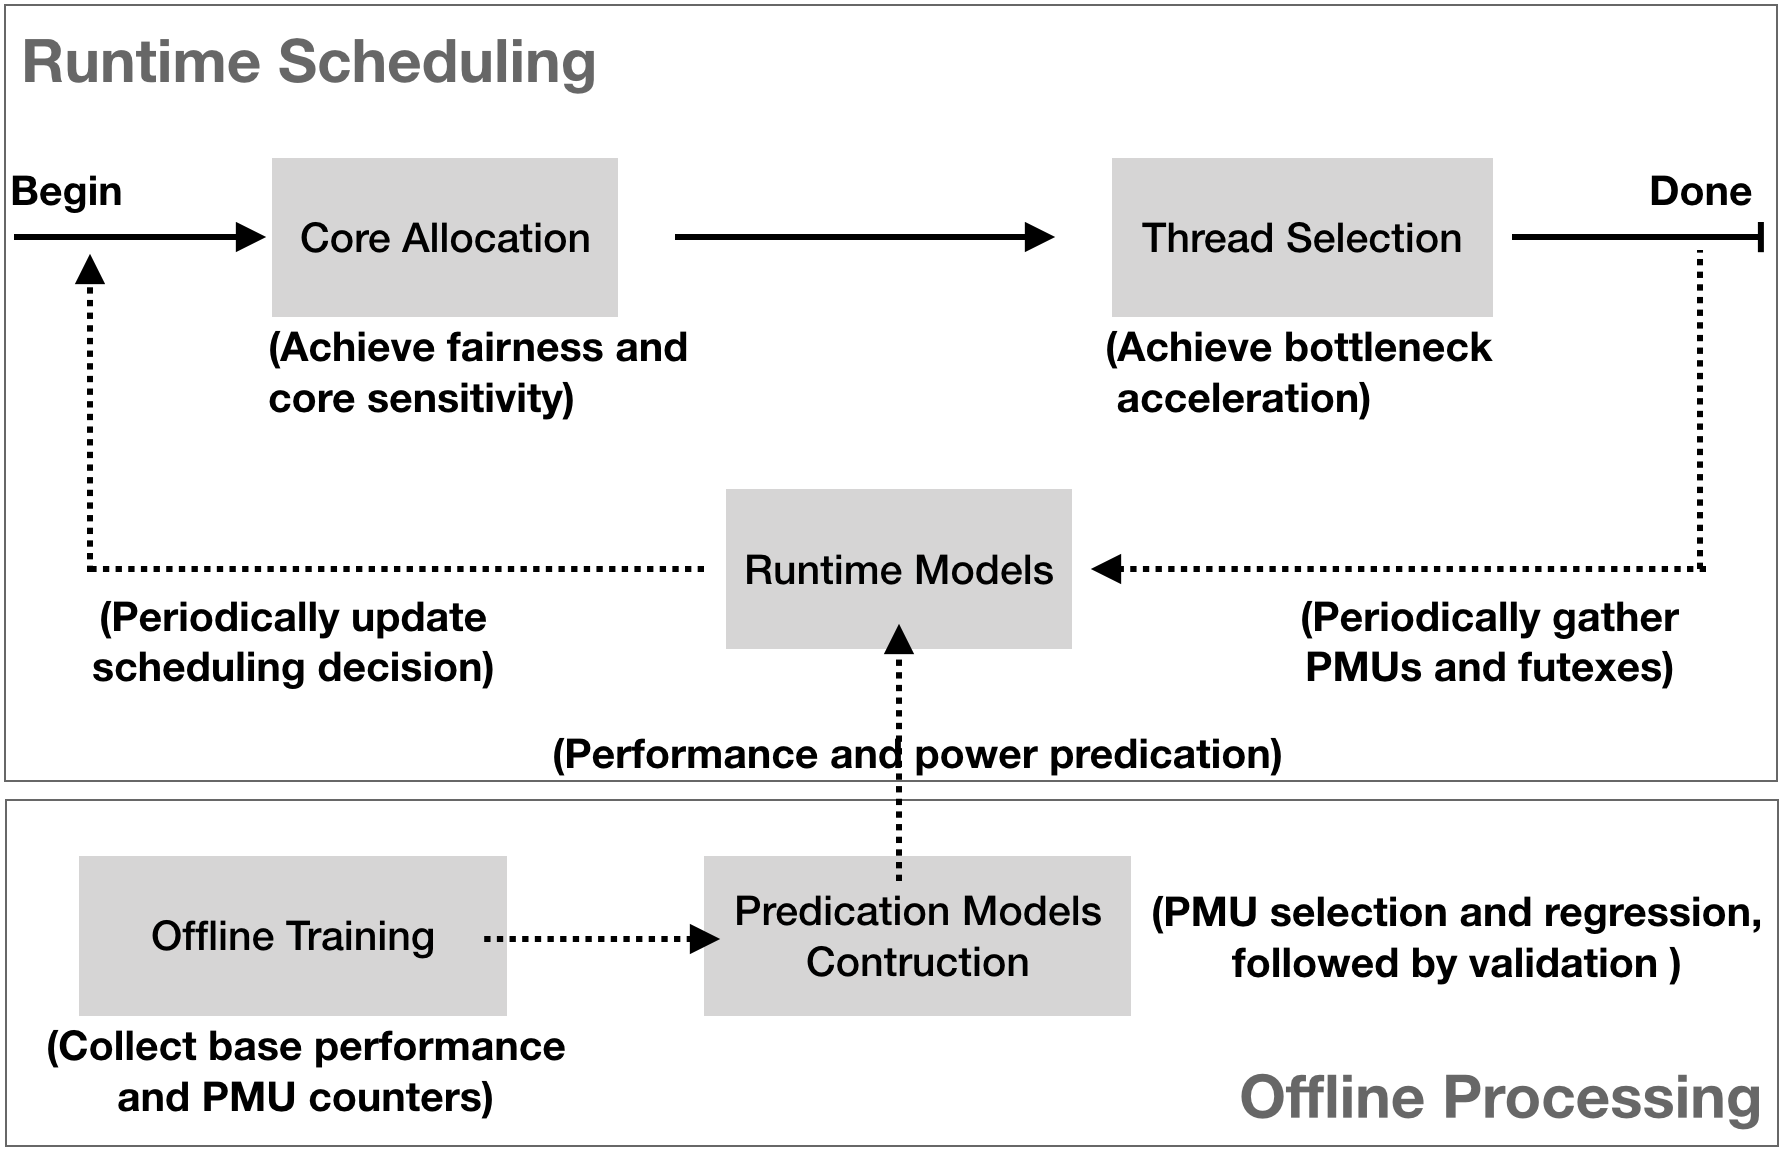
\includegraphics[scale=0.5]{figures/overview.png}
\caption{System Overview}
\label{figure:f1}
\end{figure} 

\subsection{Runtime Factor Analysis}
Figure~\ref{figure:f1} shows the relationship between runtime performance factors and the scheduler components that address them. In order to achieve runtime collaboration, both the core allocator and the thread selector share information and account for all measured performance factors, including core sensitivity, bottleneck acceleration and fairness,% carefully 
 as illustrated below:
%We describe them below by discussing each element. 
%\begin{itemize}

\textbf{\textit{Core Allocator:}}
AMP-aware Core allocators are mainly directed by the core sensitivity factor -- migrating a high speedup thread (with a large differential between big and little core execution time) from  a little core to execute on a big core will generally provide more benefit than migrating a low speedup thread. 
However this heuristic is overly simplistic. Issues are revealed when the bottleneck factor is considered simultaneously on multiprogrammed workloads. Previous approaches \cite{jibaja2016portable} simply combine the calculation from  bottleneck acceleration and predicted speedup together, but this can result in suboptimal scheduling decisions -- both locking threads and high speedup threads may be accumulating in the runqueues of big cores as described in the motivating example. More intelligent core allocation decisions can be made by avoiding a simple combination of bottleneck acceleration and speedup -- the overall schedule can benefit from a more collaborative execution environment where big cores focus on high speedup bottleneck threads, and little cores handle other low speedup bottlenecked threads without additional migration.
%migrating threads with a lower predicted speedup, but which are blocking other threads.  
Furthermore, core allocators attempt to achieve relative fairness on AMPs by efficiently sharing heterogeneous hardware and avoiding idle resources as much as possible. 
Simply mapping ready threads uniformly between different type of cores can not achieve true load-balancing -- the number of ready threads prioritized on different type of core is different and thus a hierarchical allocation should be applied to guarantee overall fairness, which avoids the need to frequently migrate threads to empty runqueues. 

\textbf{\textit{Thread Selector:}}
The \textit{thread selector} makes the final decisions on which thread will be executed during runtime. It is usually the responsibility of the thread selector to avoid bottlenecking by thread blocking. In a multi-thread multiprogrammed environment, multiple bottleneck threads from different programs may need to be accelerated simultaneously with constrained hardware resources. Instead of simply detecting the bottleneck threads and assigning all of them to big cores, as previous bottleneck acceleration schedulers do~\cite{jibaja2016portable,joao2013utility,joao2012bottleneck}, the thread selector needs to make collaborative decisions -- ideally, both big cores and little cores select bottlenecks to run simultaneously.
Core sensitivity is usually unimportant to the thread selector -- whether a thread can enjoy a high speedup from a big core compared with a little core is unrelated to which runqueue it is on, or came from. Therefore the thread selector should separate thread priority caused by core sensitivity and solely base decisions on bottleneck acceleration. One exception is that when the runqueue of a big core is empty and the thread selector is invoked -- the speedup factors from core sensitivity of ready threads should be considered only in this case. Big cores may even preempt the execution of little cores when necessary.  
The final concern of thread selector concerns fairness. Scaling time slice of threads by updating the time interval of thread selector has been shown to efficiently guarantee the equal progress \cite{van2013fairness} in multi-threaded single-program workloads and achieve fairness. 
%In single-threaded multiprogrammed scenarios, complicated fairness formulation \cite{kim2018exploring} has been proposed to guide the thread selector for more precise decisions. 
Problems occur when targeting multi-threaded multi-programmed workloads. Simply keeping a thread-level equal progress is not enough to guarantee the multi-application level fairness -- the thread selector should ensure the whole workload is in equal progress without penalizing any individual application. In fact,  multi-bottleneck acceleration by both big and little cores does provide an opportunity for this - the thread selector makes the best attempt to keep fairness on all applications by accelerating bottlenecks from all of them and as soon as possible.


%\textbf{\textit{Fairness:}} Fairness is critical for system performance. A good schedule achieving relative fairness on AMPs should efficiently share heterogeneous hardware and avoid idle resource as much as possible. To achieve the expected relative equal-progress between threads and load-balancing between cores, the core allocator should map ready threads relative uniformly,avoiding the need to frequently migrate threads to empty runqueues. The design of the preemption triggering mechanism  also affects fairness, as it determines the maximum length of a time slice.


%The preemption triggering mechanism of thread selector is also related with the fairness factor as it determines the slice of a task running each time - a thread currently running on big cores should have relatively shorter time slice against its running on little cores to result in similar progress.
%The preemption should be triggered and the thread selector should be invoked less frequent on little cores than on big cores     

%\textbf{\textit{Core Sensitivity:}} Previous approaches considered core sensitivity and predicated speedup of threads but can result in poor scheduling decisions on multi-threaded, multi-programmed co-execution workloads. Selecting threads simply by predicted speedup on asymmetric cores may not lead to a overall good solution --  for instance, a high speedup thread detected on a little core could benefit by migrating to a big core, but is not blocking a significant number of other threads. The overall schedule can benefit more by migrating threads with a lower predicted speedup, but which are blocking other threads. Thus, we find priority from core sensitivity should be mainly addressed by the core allocator and be independent from the thread selector. 
%For instance, a thread with high predicted speedup should have more opportunities to be allocated and executed on a high-performance big core compared to a low predicted speedup thread. Higher speedup and more sensitive on big core does not indicate any {\it emergency} to execute this threads amount all other ready threads during the runtime. 
%No priority should be given to high-speedup threads for a thread selector, only if in a special case when a big core finishes its current task with an empty runqueue and all other big cores hold empty runqueue as well - so it needs to globally select a ready thread from a runqueue of little core and then relative higher speedup threads are better candidates. This special case won't even appear in large-scale parallel workloads scenarios where the number of co-executing programs is at least greater than the number of cores - there will always be waiting threads in a big core's runqueue based on fairness core allocation as no data-dependence between threads from different programs. 

%\textbf{\textit{Bottleneck Acceleration:}} Threads from multi-threaded programs holding contended locks and blocking other parallel threads should be identified as bottleneck and be executed as soon as possible. In large-scale workloads scenarios where multi-threaded multi-program are co-executing on limited AMPs resources and multiple blocking threads waiting to be executed simultaneously, the thread selector should take the main duty to select those bottlenecks and run the corresponding critical code segments in an efficient way without confused by the priority from core sensitivity. In detail, the thread selector triggered by big cores should always give higher priorities for a thread with higher blocking level against another thread with higher speedup level and lower bottleneck. It may preempt the running threads on little cores to accelerate them when suited. The thread selector triggered by little cores should also intend to select relative high blocking threads and accelerate them locally first, instead of trivially migrating it to big cores and waiting to be actual accelerated there.  

\begin{figure}
\centering
\includegraphics[scale=0.5]{figures/COLAB_M.pdf}
\caption{Coordinated Runtime Scheduling by Multi-factor Collaboration}
\label{figure:f2}
\end{figure} 

\subsection{Collaboration}
To address the problems detailed above, we designed a coordinated multi-factor scheduler in which the core allocator and the thread selector collaborate to achieve high performance and high fairness, when compared to %the state-of-the-art mixed multi-factor evaluator in 
WASH \cite{jibaja2016portable}.
% VJ " We mentioned quite a few times already that WASH is state-of-the-art mixed multi-factor thing...
%While the way we define whether a thread's relative speedup value is high or low is similar as in WASH based on hardware configuration - if we have same number of big and little cores, then we rank all ready threads based on its relative speedup and view the first half as high speedup value. 
The flowchart of our model is shown in Figure~\ref{figure:f2}. 
Collaboration is facilitated by periodically labeling ready threads in two different categories, based on runtime models of speedup prediction and bottleneck identification: 
%\begin{itemize}

\textbf{\textit{Labels for Core Allocation:}}
Threads with high predicted speedup between big and little cores will be labeled as high priority on big cores. Threads with both low predicted speedup and blocking levels -- non-critical threads -- will obtain high priority on little cores (and low priority on big cores). Remaining threads obtain equal priority on either big or little cores -- these threads can then be allocated freely to balance the load of cores.

\textbf{\textit{Labels for Thread Selection:}}
Threads with high blocking level will be labeled as high priority on local thread selection. The same priority will be given on these blocking threads whether the issuing cores are big or little, so the labels of thread selection do not distinguish the type of cores.The label nevertheless records the type of the current core -- threads always have priority to be selected by the same type of cores if there exists a core of the same type with an empty runqueue. Running threads on little cores are also labeled as they may be preempted to migrate and execute on big cores when suited, but running threads will never have priority over waiting ready threads. 


%The thread labels should be not only be based on the relative ranking between threads, but also on boundary conditions targeting different hardware resource and experimental environments. 
%We setup empirical boundaries for speedup and blocking: (1) No thread is ranked as high-speedup if its predicted speedup value is less than an empirical architecture-specific boundary, calculated using relative frequency between big and little cores. 

%For instance, if the big cores' frequency is 2x faster than the little cores and ready threads get around 1.5x predicted speedup, this likely means threads haven't be executed long enough to get a more precise speedup value and we should not bind or migrate any thread at this step. 
%(2) Threads will not be ranked as high-blocking if the rate of their blocking time and life time are less than a relative boundary or the life time of them are less than a starting point - For instance, no thread should be ranked as relative high-blocking during the initial time periods of experiments.   
%It is mainly benefit in a mixed workloads scenario where we co-execute single and multi-threaded multiprogrammed - a non-computing-intensive code segment from a single thread program can neither enjoy good performance gain on big cores nor block others. So we should better keep it in a little core and let other blocking threads to be executed before it. 

After the labeling process, fairness, core sensitivity and bottleneck acceleration are represented by labels on threads can be handled by either the core allocator or the thread selector or both together. Based on this coordinated model, the core allocator and thread selector handle different priorities queues from the set of ready threads -- their decisions are not greedy on a mixed multi-factor ranking like WASH, rather provide a collaborative schedule.
Another important issue handled by the collaborative multi-factor model is to ensure equal-progress of threads as shown in the upper-right corner of Figure~\ref{figure:f2}. Instead of interfering with the priority and decisions of thread selection, we achieve equal progress in threads by our scaled time slice approach, based on the predicted speedup value of threads running on big cores. The slices of threads on big cores are relative shorter than on little cores. The thread selection function is triggered more often to swap executing threads on big cores, which guarantees the relative equal-progress of threads executed on all cores.
The runtime model periodically extracts the performance counters, which represents the current execution environment of multi-threaded multi-programmed workloads on the AMPs. The model then computes the updated runtime factors, including the predicated speedup value and blocking counts. This information is attached to the threads and reported back to the multi-factor labeler for next round. We present our runtime implementations in the section below. 

\section{Scheduler Design and Implementation on GEM5}
We first implement our prototype scheduler on the GEM5 simulator. \cite{binkert2011gem5}
%and the Linux kernel v3.16.
%with the CFS scheduler. 
\vspace{-1em}
\subsection{COLAB Runtime Implementations}
To implement the runtime multi-factor model, we update the main scheduler function \texttt{\_\_sched\_\_schedule()} of the Linux kernel by adding a thread labeling process as described in section 3.2 above. A similar approach is followed by our WASH re-implementation when updating thread affinities.

\textbf{\textit{Machine Learning based Speedup and Energy Prediction:}} 
Predicting the relative speedup of each thread between different core types is central for any scheduler targeting AMPs. Our prediction uses an offline trained speedup model to estimate speedups online. This is a common approach in previous works \cite{van2013fairness,jibaja2016portable,saez2012leveraging}.
To construct the training set, we run all applications in single-program mode with two symmetric configurations, using either only little cores or only big cores. We first record all counters of the big cores and the relative speedup between the two configurations. Since the targeting ARM architecture only contains 7 hardware register to support performance monitor units (PMUs), we do not have access to all PMUs simultaneously. We apply Principal Component Analysis (PCA) technique \cite{witten2016data} to select the 6 performance counters with the largest effect on speedup modeling, together with the counter on committed instructions. We then normalize all counters to the number of committed instructions on GEM5 and use linear regression to build the final model. 
%The selected counters and speedup model targeting the GEM5 is shown in Table \ref{pca_gem5_sp}. 


\begin{comment}
\begin{table}
  \caption{Selected GEM5 performance counters and the Speedup Model}
  \center
  \label{pca_gem5_sp}
   \scalebox{0.8}{
   \begin{tabular}{p{0.8cm} | p{4.8cm} | p {3.8cm} c c c}
  \hline
     Index&  Name& Description \cite{binkert2011gem5} \\
    \hline
     A: & fp\_regfile\_writes & \# integer regfile writes\\
     B: & fetch.Branches & \# branches encountered\\
     C: & rename.SQFullEvents & \# SQ-full blocks\\
     D: & quiesceCycles & \# interrupt waiting cycles\\
     E: & dcache.tags.tagsinuse & \# tags of dcache in use\\
     F: & fetch.IcacheWaitRetryStallCycles & \# MSHR-full stall cycles\\
     \hline
     G: & commit.committedInsts & \# instructions committed\\
     \hline
     \multicolumn{3}{c}{Linear predictive speedup model}\\
     \hline
    \multicolumn{3}{c}{2.6109+((0.0018*-0.185A)+(0.0259*0.187B)+}
    \\
    \multicolumn{3}{c}{(0.1047*0.194C)+(-0.023*0.238D)+(0.0492*-0.299E)+(-0.1388*-0.227F))/G}\\
 \hline
  \end{tabular}}
\end{table}
\end{comment}

\textbf{\textit{Bottleneck Identification:}}
On modern Linux systems synchronization primitives are almost always implemented using kernel futexes, regardless of the threading library used. Futex-based mechanisms use a single atomic instruction in user space to acquire or release the futex, if it is uncontested. Otherwise, it triggers system calls to forces the thread to sleep or to wake up sleeping threads.
This gives us a convenient single point for monitoring blocking patterns between threads. We first add code in \texttt{futex\_wait\_queue\_me()} and \texttt{futex\_lock\_pi()}, right before the active thread starts waiting on a futex. We record the current time and store it in the \texttt{task\_struct} of the thread. We then insert code in \texttt{wake\_futex()} and \texttt{wake\_futex\_pi()}, right before the waiting task is woken up by the thread releasing the futex. There we calculate the length of the waiting period and we accumulate it in the \texttt{task\_struct} of the thread releasing the futex. This way we are able to measure the cumulative time each thread has caused other threads to wait. We use this as our metric of thread criticality for the rest of the paper.

\textbf{\textit {Speedup based Scale-slice Preemption:}} Although we implement our scheduler on Linux kernel by fully re-writing both the core allocator and thread selector, the underlining preemption mechanism of Linux is applying the virtual runtime {\it vruntime} in CFS with red-black tree data structure - whenever a new task is enqueued, a preemption wake-up function is invoked to check whether the new coming task should preempt the current task by computing the difference in vruntime and comparing with a boundary. 
To achieve equal-progress on AMPs, threads running on different types of cores should have different time slices instead of trying to achieve complete fairness on time. We update the default preemption function \texttt{wakeup\_preempt\_entity()} in Linux. To ensure relative equal progress, we apply our runtime speedup model to update the vruntime of the task by dividing it by the its speedup value if the triggering core is a big core. %The ensures relative equal progress.




\subsection{COLAB Algorithm Implementation}
\begin{algorithm}
\caption{COLAB: Collaborative Multi-factor Scheduler targeting Asymmetric Multicore Processors}
\label{alg:1}
\begin{algorithmic}[]
\STATE \textbf{\_core\_alloctor\_(thread\_struct\ $t$)}\{
%\FOR {$t : ready\_threads$}
%\IF {t->high\_speedup() \& t->high\_block()}
%\STATE \textbf{if} foo

%\IF {t.high\_speedup}
%\RETURN rr\_allocator\_(big\_cores)
%\ENDIF
\STATE \textbf{if} t.high\_speedup
\STATE \ \ \textbf{return} rr\_allocator\_(big\_cores)
\STATE \textbf{if} {t.low\_speedup \& t.low\_block}
\STATE \ \ \textbf{return} rr\_allocator\_(little\_cores)

\STATE \textbf{else return} rr\_allocator\_(cores) \}
\STATE
\STATE \textbf{\_thread\_selector\_(core\_struct\ $c$)}\{
%\IF {c->cur \& !(preempt_wakeup)}
\STATE \textbf{if}  !empty(c.rq)
\STATE \ \ \textbf{return} max\_block\_(c.rq)
\STATE \textbf{if} !empty(c.sched\_domain.rq)
\STATE \ \ \textbf{return} max\_block\_(c.sched\_domain.rq)
\STATE \textbf{if} c.cpu\_mask == big
%\FOR {t : little\_core->cur}
%\STATE candidates.enqueue(t)
%\IF {!empty(candidates)}
\STATE \ \ \textbf{return}  max\_block\_(c.sched\_domain\_little.cur)
%\ENDFOR
%\ENDIF
%\FOR {t : other\_little\_core->rq}
%\STATE candidates.enqueue(sorted\_speedup(t))
%\ENDFOR
%\IF {!empty(candidates)}
%\RETURN  max\_block\_(candidates)
%\ENDIF
%\ENDIF
%\FOR {t : other\_core->rq}
%\STATE candidates.enqueue(reversed\_speedup(t))
%\ENDFOR
\STATE \textbf{else return} idle \}
\end{algorithmic}
\end{algorithm}

\noindent
Our scheduling algorithm (see Alg.~\ref{alg:1}) is implemented by overriding the default task selector \texttt{pick\_next\_task\_fair()} and core allocator \texttt{select\_task\_rq\_fair()} in Linux kernel supported by the runtime factors. %The pseudo-code of our scheduling algorithm is shown in Alg. \ref{alg:1}. 
In line with standard Linux notation, we use $rq$ and $cur$ to represent runqueue and the current task of a core, respectively. We describe the two main functions followed by a discussion on scheduling overhead:

\textbf{\textit{Hierarchical Core Allocator:}}
When a spawned or woken thread is ready to be executed, the core allocator will be invoked to assign this thread to a core's runqueue. To achieve relative load balancing and consider the influence from the core sensitivity factor, we involve a hierarchical round-robin mechanism \texttt{rr\_allocator\_()}. Indicated by the speedup and blocking labels, threads are allocated to different core groups. Threads with high speedup will be round-robin assigned in big core clusters. Low speedup and low blocking threads will only be assigned in little core clusters. 
%A technical issue here is we need to distinguish threads which are part of a multi-thread program from from single-thread programs - these single-thread program threads will definitely not block others and may not have a high speedup but we should nevertheless not bind them to little cores. They can be easily detected by the allocator by checking whether there are ready threads whose group pid (t->tgid) equals to any others (line 5). 
Remaining ready threads (usually with average speedup level and little blocking) will be relatively equally allocated to both core types by \texttt{rr\_allocator\_()}. This final round-robin decision helps to keep both core clusters equally occupied and load balanced. 

\textbf{\textit{Biased-global Thread Selector:}}
The thread selector is based on the principle of accelerating the most critical/blocking thread as soon as possible. The selector always tries to choose a thread from the local runqueue first. When there are no ready threads and migration is beneficial, the core triggers the migration of a candidate thread waiting in another runqueue. The highest blocking thread will be selected.
To reduce the overhead of accessing state in other runqueues, we follow the same principle as the default Linux CFS scheduler, returning the best candidate thread from the local core group first.
Further, we allow a big core to select and preempt a running thread on a little core to accelerate it. Big cores are allowed to go idle only when there is no ready thread left - for instance, we do not allow a little core to preempt a big core's execution. 
%In summary, the thread selector can still access all other runqueues when necessary, but it is biased to access neighbouring ones first. 
The equal-progress for achieving fairness is addressed by the scale-slice preemption checker  -- we give each thread a maximum time slice relative to its expected performance on the asymmetric core.



